\documentclass[tikz,convert={outfile=foldNatFree-mmorph-join.svg}]{standalone}
\begin{document}
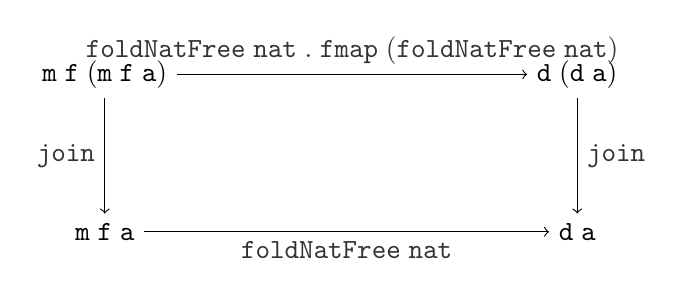
\begin{tikzpicture}
    \node (A) at (0,2) {\texttt{$\mathtt{m}\;\mathtt{f}\;(\mathtt{m}\;\mathtt{f}\;\mathtt{a})$}};
    \node (B) at (6,2) {\texttt{$\mathtt{d}\;(\mathtt{d}\;\mathtt{a})$}};
    \node (C) at (0,0) {\texttt{$\mathtt{m}\;\mathtt{f}\;\mathtt{a}$}};
    \node (D) at (6,0) {\texttt{$\mathtt{d}\;\mathtt{a}$}};
    \draw[->] (A) -- node[above]
    {\textcolor{black!80}{$\mathtt{foldNatFree}\;\mathtt{nat}\;.\;\mathtt{fmap}\;(\mathtt{foldNatFree}\;\mathtt{nat})$}} (B);
    \draw[->] (B) -- node[right] {\textcolor{black!80}{$\mathtt{join}$}} (D);
    \draw[->] (A) -- node[left] {\textcolor{black!80}{$\mathtt{join}$}} (C);
    \draw[->] (C) -- node[below] {\textcolor{black!80}{$\mathtt{foldNatFree}\;\mathtt{nat}$}} (D);
\end{tikzpicture}
\end{document}

